% Draft captions for the three main-text figures.
% Usage: % Draft captions for the three main-text figures.
% Usage: % Draft captions for the three main-text figures.
% Usage: % Draft captions for the three main-text figures.
% Usage: \input{figures/captions} is not intended; copy each \caption into its figure environment.
% Cite keys refer to arxiv/references.bib.

% ---------------------------------------------------------------- Fig. 1
\begin{figure}[tbp]
\centering
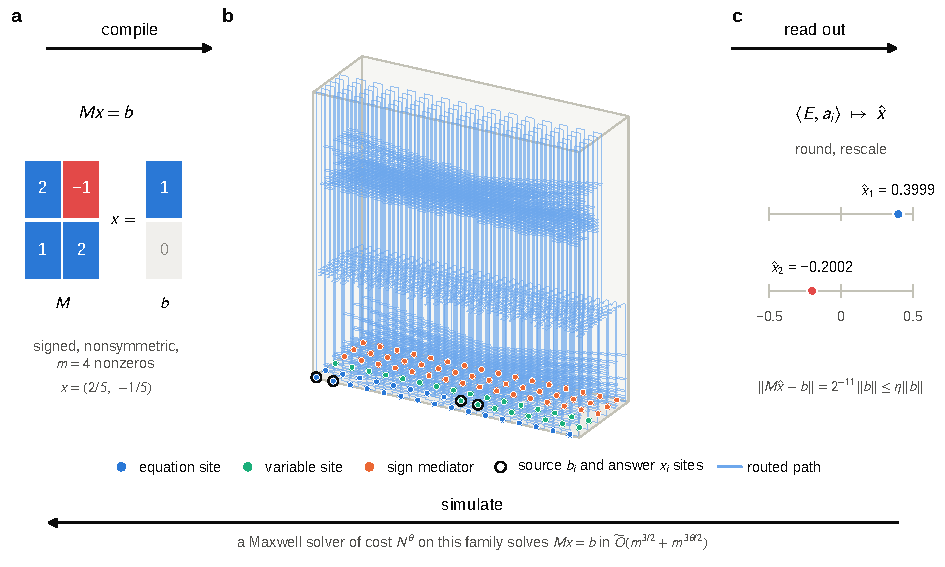
\includegraphics[width=\linewidth]{figures/fig1_concept.pdf}
\caption{\textbf{A sparse linear system and a dielectric cavity encode each other.}
\textbf{a}, The input is a sparse system $Mx=b$ with $m$ signed rational coefficients; shown is the
$2\times2$ example $M=\bigl(\begin{smallmatrix}2&-1\\1&2\end{smallmatrix}\bigr)$, $b=(1,0)$, whose
solution is $x=(2/5,\,-1/5)$. Blue and red cells are positive and negative entries.
\textbf{b}, The compiler expresses the equations through a local network of 96 sites (equation sites,
variable sites and sign mediators, each connected to at most three others) and routes its 96
connections as paths through a $505\times169\times3105$ integer grid. The drawing is the network the
compiler produced for the example in a, with the routing axis compressed sixfold for display; the paths
are long because the compiler equalizes their lengths. Each site becomes a broad, weak defect in the
periodic dielectric that fills the box, each path becomes a chain of such defects, and the walls are
perfect conductors. Ringed sites carry the source $b$ and the answer $x$.
\textbf{c}, A finite list of field moments $\langle E,a_i\rangle$ at the answer sites, rounded and
rescaled, returns $\hat x$. For the example, exact arithmetic on the compiled network gives
$\hat x=(819/2048,\,-205/1024)$ with relative residual $2^{-11}$, within the requested tolerance
$\eta=1/4$. Read from left to right (compile, read out), the cavity is an optical computer for $Mx=b$;
read from right to left (simulate), a Maxwell solver that handles this family of cavities in time
$N^{\theta}$, where $N$ counts grid cells, is a sparse linear solver of cost
$\widetilde O(m^{3/2}+m^{3\theta/2})$.}
\label{fig:concept}
\end{figure}

% ---------------------------------------------------------------- Fig. 2
\begin{figure}[tbp]
\centering
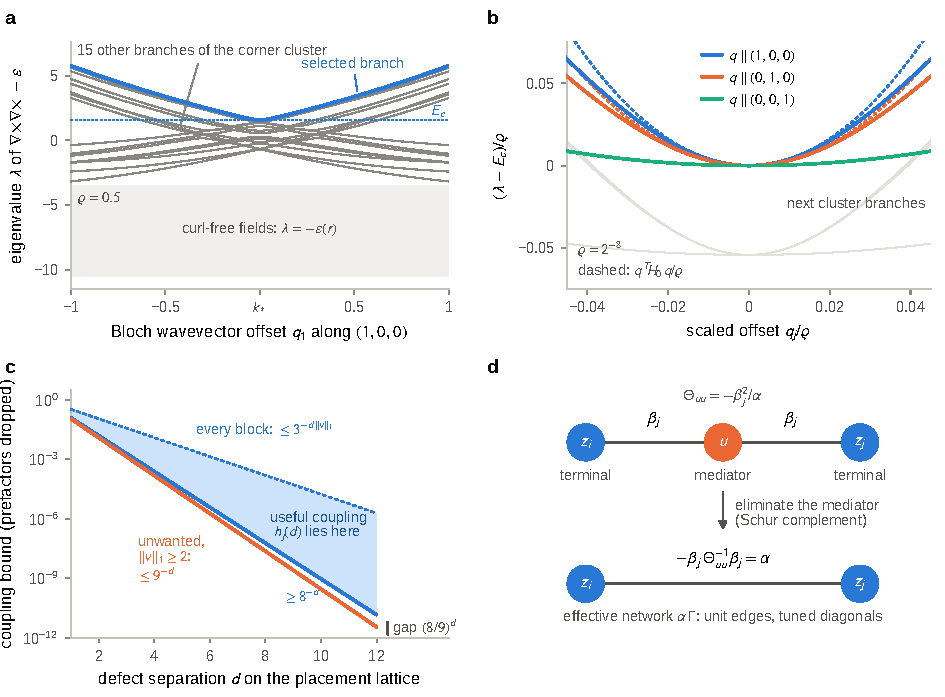
\includegraphics[width=\linewidth]{figures/fig2_mechanism.pdf}
\caption{\textbf{Broad defects in a weakly modulated dielectric interact like a network.}
\textbf{a}, Bloch spectrum of $\nabla\times\nabla\times-\varepsilon(x)$ for the periodic background
$\varepsilon=7+\delta\,[\cos\pi x_1+2\cos\pi x_2+4\cos\pi x_3]$ along the line $k=k_*+q_1(1,0,0)$
through $k_*=(\pi/2,\pi/2,\pi/2)$, computed with a vector plane-wave expansion (1029 plane-wave
components; eigenvalues converged to $10^{-7}$). The modulation is exaggerated to $\delta=0.5$ for
visibility; the construction uses $\delta=2^{-100}$. At $k_*$ eight plane waves of the unmodulated
medium are degenerate, forming a cluster of sixteen transverse branches that the modulation splits.
The selected branch (blue) is the highest of them and has an isolated local minimum $E_c$ at $k_*$.
Curl-free fields contribute the band $\lambda=-\varepsilon(x)$ (gray), and the other cluster branches
cross $E_c$ away from $k_*$: there is no complete gap, and the proof bounds leakage into these states
instead of assuming its absence.
\textbf{b}, The selected branch near $k_*$ along the three axes, computed at $\delta=2^{-8}$ and drawn
in scaled variables, in which the curves no longer change as $\delta\to0$. Dashed: the quadratic form
$q^{T}\!A_0\,q/\delta$ with the exact leading-order Hessian of the proof,
$A_0=\pi^2\,\mathrm{diag}(4.12,\,3.26,\,0.44)$; the next branches of the cluster (light gray) stay
$0.054\,\delta$ below the minimum.
\textbf{c}, Proven decay rates of the interaction between two defects $d$ placement-lattice steps
apart, with constant prefactors dropped: the useful nearest-neighbor coupling $h_j(d)$ is at least
$8^{-d}$ and, like every interaction block, at most $3^{-d}$, whereas every block between defects
that are not nearest neighbors is at most $9^{-d}$. The gap between the two rates is $(8/9)^{d}$:
because $9>8$, the summed unwanted couplings fall below the useful ones once $d=O(\log m)$.
\textbf{d}, A sign mediator $u$ between two terminals $z_i$, $z_j$ with couplings $\beta_j$ and tuned
self-term $T_{uu}=-\beta_j^2/\alpha$; eliminating it leaves the effective coupling $\alpha$, so the
defect amplitudes obey $\alpha\Gamma z=\alpha g$ for the compiled network matrix $\Gamma$, which has
unit edges and tuned diagonals.}
\label{fig:mechanism}
\end{figure}

% ---------------------------------------------------------------- Fig. 3
\begin{figure}[tbp]
\centering
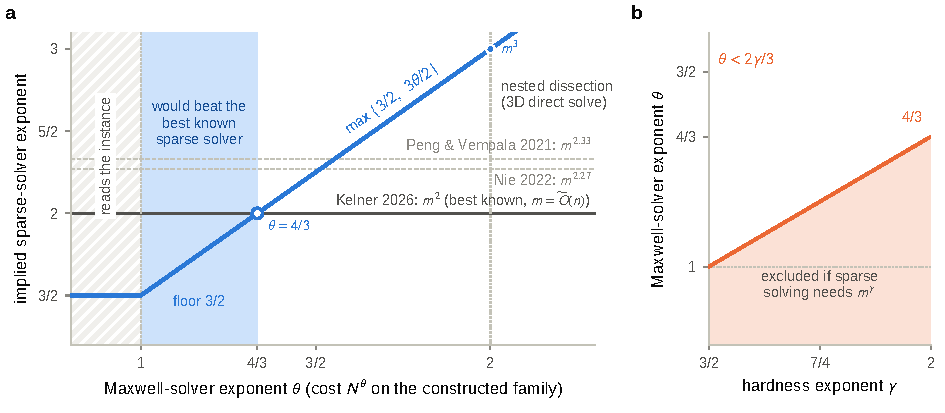
\includegraphics[width=\linewidth]{figures/fig3_consequence.pdf}
\caption{\textbf{What a fast Maxwell solver would mean for sparse linear algebra.}
\textbf{a}, If a solver handles every cavity of the constructed family in time $N^{\theta}$ up to
logarithmic factors, where $N$ counts grid cells and description length, then encoding, solving and
decoding solve every polynomially conditioned sparse system with $m$ nonzeros in time
$m^{\max\{3/2,\,3\theta/2\}}$ up to logarithmic factors (blue; the floor $3/2$ is the cost of encoding
and decoding). Horizontal lines are known bit-complexity upper bounds for the same problem class
($m=\widetilde O(n)$ nonzeros, polynomial condition number): the
$\widetilde O(mn\log(\kappa/\epsilon))$ algorithm of Kelner~\cite{kelner2026} gives $m^{2}$ and
supersedes the $m^{2.33}$ of Peng and Vempala~\cite{pengvempala2021,PengVempala2025} and the
$m^{2.27}$ of Nie~\cite{nie2022} (both stated with the matrix-multiplication exponent $\omega<2.3729$
used in those papers). Vertical
lines mark $\theta=1$, below which a solver can not read its input, and $\theta=2$, the cost of a
nested-dissection direct solve on a three-dimensional grid~\cite{George1973,LiptonRoseTarjan1979}. A
uniform solver with $1\le\theta<4/3$ (shaded) would improve the best known sparse-solver exponent.
The statement concerns worst-case solvers on this family of cavities; it says nothing about solvers
for other geometries or about typical instances.
\textbf{b}, Conversely, if solving sparse systems requires time $m^{\gamma}$ for some
$\gamma\in(3/2,2]$, the range compatible with the $m^{2}$ upper bounds (conjugate gradients in exact
arithmetic in the real-arithmetic model of the hypothesis; Kelner's algorithm in the bit model), no
uniform Maxwell solver for the family can have $\theta<2\gamma/3$ (shaded).}
\label{fig:consequence}
\end{figure}
 is not intended; copy each \caption into its figure environment.
% Cite keys refer to arxiv/references.bib.

% ---------------------------------------------------------------- Fig. 1
\begin{figure}[tbp]
\centering
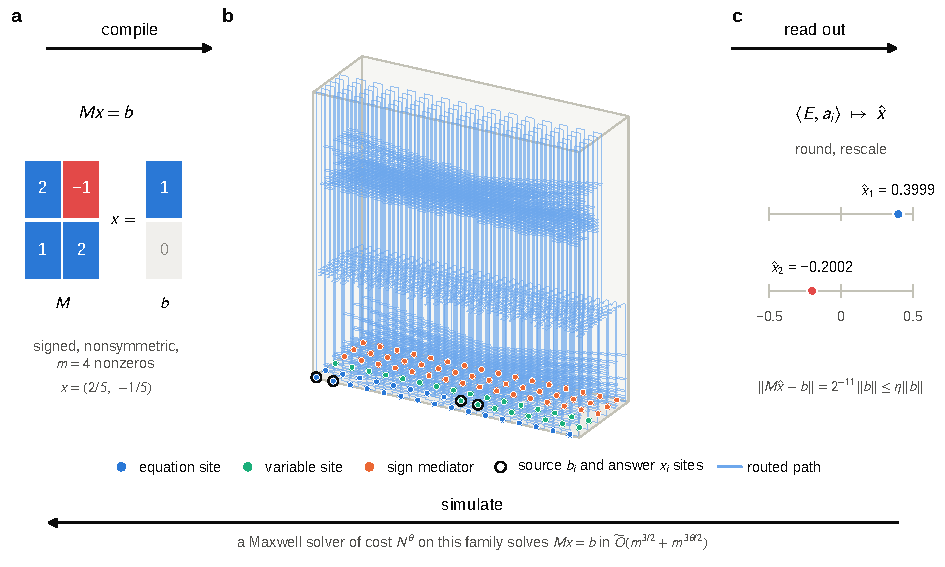
\includegraphics[width=\linewidth]{figures/fig1_concept.pdf}
\caption{\textbf{A sparse linear system and a dielectric cavity encode each other.}
\textbf{a}, The input is a sparse system $Mx=b$ with $m$ signed rational coefficients; shown is the
$2\times2$ example $M=\bigl(\begin{smallmatrix}2&-1\\1&2\end{smallmatrix}\bigr)$, $b=(1,0)$, whose
solution is $x=(2/5,\,-1/5)$. Blue and red cells are positive and negative entries.
\textbf{b}, The compiler expresses the equations through a local network of 96 sites (equation sites,
variable sites and sign mediators, each connected to at most three others) and routes its 96
connections as paths through a $505\times169\times3105$ integer grid. The drawing is the network the
compiler produced for the example in a, with the routing axis compressed sixfold for display; the paths
are long because the compiler equalizes their lengths. Each site becomes a broad, weak defect in the
periodic dielectric that fills the box, each path becomes a chain of such defects, and the walls are
perfect conductors. Ringed sites carry the source $b$ and the answer $x$.
\textbf{c}, A finite list of field moments $\langle E,a_i\rangle$ at the answer sites, rounded and
rescaled, returns $\hat x$. For the example, exact arithmetic on the compiled network gives
$\hat x=(819/2048,\,-205/1024)$ with relative residual $2^{-11}$, within the requested tolerance
$\eta=1/4$. Read from left to right (compile, read out), the cavity is an optical computer for $Mx=b$;
read from right to left (simulate), a Maxwell solver that handles this family of cavities in time
$N^{\theta}$, where $N$ counts grid cells, is a sparse linear solver of cost
$\widetilde O(m^{3/2}+m^{3\theta/2})$.}
\label{fig:concept}
\end{figure}

% ---------------------------------------------------------------- Fig. 2
\begin{figure}[tbp]
\centering
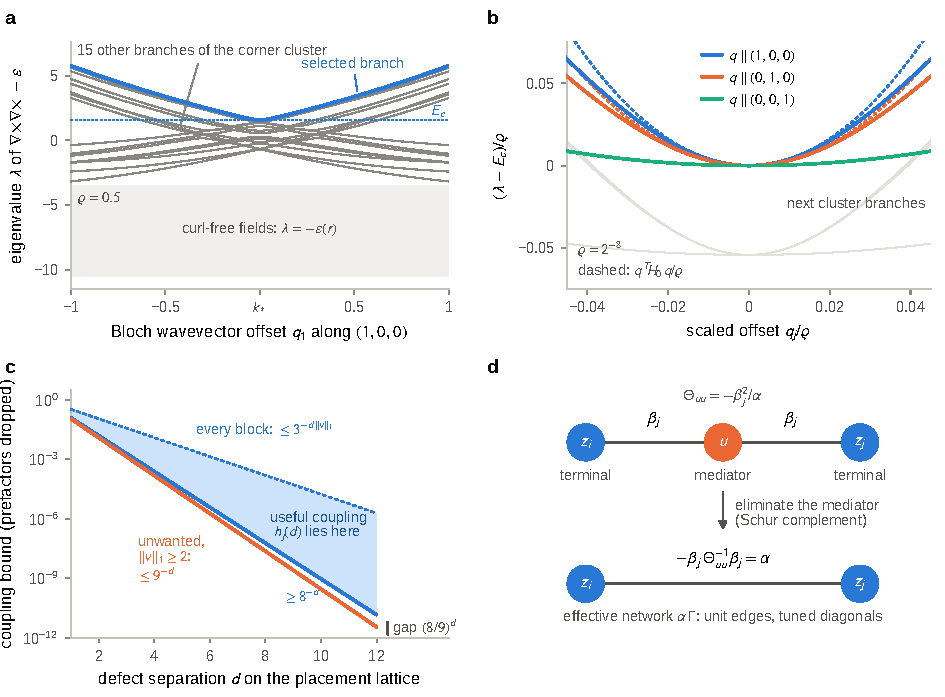
\includegraphics[width=\linewidth]{figures/fig2_mechanism.pdf}
\caption{\textbf{Broad defects in a weakly modulated dielectric interact like a network.}
\textbf{a}, Bloch spectrum of $\nabla\times\nabla\times-\varepsilon(x)$ for the periodic background
$\varepsilon=7+\delta\,[\cos\pi x_1+2\cos\pi x_2+4\cos\pi x_3]$ along the line $k=k_*+q_1(1,0,0)$
through $k_*=(\pi/2,\pi/2,\pi/2)$, computed with a vector plane-wave expansion (1029 plane-wave
components; eigenvalues converged to $10^{-7}$). The modulation is exaggerated to $\delta=0.5$ for
visibility; the construction uses $\delta=2^{-100}$. At $k_*$ eight plane waves of the unmodulated
medium are degenerate, forming a cluster of sixteen transverse branches that the modulation splits.
The selected branch (blue) is the highest of them and has an isolated local minimum $E_c$ at $k_*$.
Curl-free fields contribute the band $\lambda=-\varepsilon(x)$ (gray), and the other cluster branches
cross $E_c$ away from $k_*$: there is no complete gap, and the proof bounds leakage into these states
instead of assuming its absence.
\textbf{b}, The selected branch near $k_*$ along the three axes, computed at $\delta=2^{-8}$ and drawn
in scaled variables, in which the curves no longer change as $\delta\to0$. Dashed: the quadratic form
$q^{T}\!A_0\,q/\delta$ with the exact leading-order Hessian of the proof,
$A_0=\pi^2\,\mathrm{diag}(4.12,\,3.26,\,0.44)$; the next branches of the cluster (light gray) stay
$0.054\,\delta$ below the minimum.
\textbf{c}, Proven decay rates of the interaction between two defects $d$ placement-lattice steps
apart, with constant prefactors dropped: the useful nearest-neighbor coupling $h_j(d)$ is at least
$8^{-d}$ and, like every interaction block, at most $3^{-d}$, whereas every block between defects
that are not nearest neighbors is at most $9^{-d}$. The gap between the two rates is $(8/9)^{d}$:
because $9>8$, the summed unwanted couplings fall below the useful ones once $d=O(\log m)$.
\textbf{d}, A sign mediator $u$ between two terminals $z_i$, $z_j$ with couplings $\beta_j$ and tuned
self-term $T_{uu}=-\beta_j^2/\alpha$; eliminating it leaves the effective coupling $\alpha$, so the
defect amplitudes obey $\alpha\Gamma z=\alpha g$ for the compiled network matrix $\Gamma$, which has
unit edges and tuned diagonals.}
\label{fig:mechanism}
\end{figure}

% ---------------------------------------------------------------- Fig. 3
\begin{figure}[tbp]
\centering
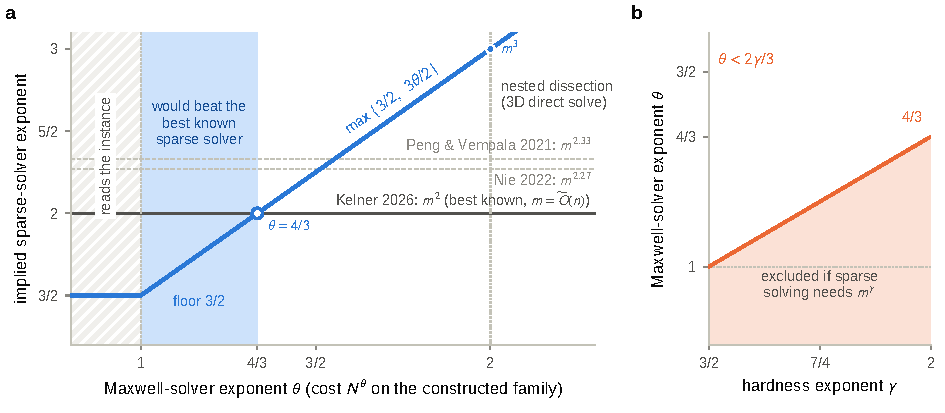
\includegraphics[width=\linewidth]{figures/fig3_consequence.pdf}
\caption{\textbf{What a fast Maxwell solver would mean for sparse linear algebra.}
\textbf{a}, If a solver handles every cavity of the constructed family in time $N^{\theta}$ up to
logarithmic factors, where $N$ counts grid cells and description length, then encoding, solving and
decoding solve every polynomially conditioned sparse system with $m$ nonzeros in time
$m^{\max\{3/2,\,3\theta/2\}}$ up to logarithmic factors (blue; the floor $3/2$ is the cost of encoding
and decoding). Horizontal lines are known bit-complexity upper bounds for the same problem class
($m=\widetilde O(n)$ nonzeros, polynomial condition number): the
$\widetilde O(mn\log(\kappa/\epsilon))$ algorithm of Kelner~\cite{kelner2026} gives $m^{2}$ and
supersedes the $m^{2.33}$ of Peng and Vempala~\cite{pengvempala2021,PengVempala2025} and the
$m^{2.27}$ of Nie~\cite{nie2022} (both stated with the matrix-multiplication exponent $\omega<2.3729$
used in those papers). Vertical
lines mark $\theta=1$, below which a solver can not read its input, and $\theta=2$, the cost of a
nested-dissection direct solve on a three-dimensional grid~\cite{George1973,LiptonRoseTarjan1979}. A
uniform solver with $1\le\theta<4/3$ (shaded) would improve the best known sparse-solver exponent.
The statement concerns worst-case solvers on this family of cavities; it says nothing about solvers
for other geometries or about typical instances.
\textbf{b}, Conversely, if solving sparse systems requires time $m^{\gamma}$ for some
$\gamma\in(3/2,2]$, the range compatible with the $m^{2}$ upper bounds (conjugate gradients in exact
arithmetic in the real-arithmetic model of the hypothesis; Kelner's algorithm in the bit model), no
uniform Maxwell solver for the family can have $\theta<2\gamma/3$ (shaded).}
\label{fig:consequence}
\end{figure}
 is not intended; copy each \caption into its figure environment.
% Cite keys refer to arxiv/references.bib.

% ---------------------------------------------------------------- Fig. 1
\begin{figure}[tbp]
\centering
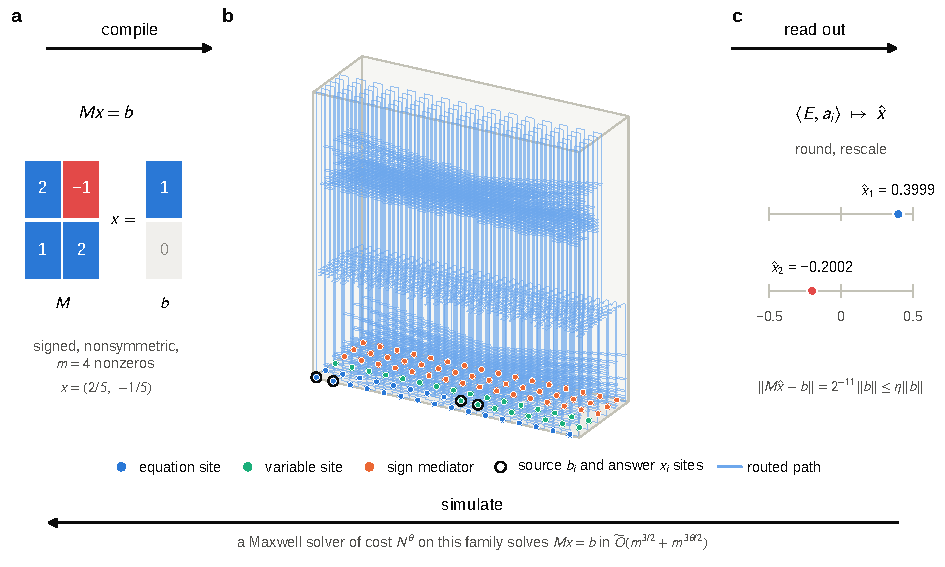
\includegraphics[width=\linewidth]{figures/fig1_concept.pdf}
\caption{\textbf{A sparse linear system and a dielectric cavity encode each other.}
\textbf{a}, The input is a sparse system $Mx=b$ with $m$ signed rational coefficients; shown is the
$2\times2$ example $M=\bigl(\begin{smallmatrix}2&-1\\1&2\end{smallmatrix}\bigr)$, $b=(1,0)$, whose
solution is $x=(2/5,\,-1/5)$. Blue and red cells are positive and negative entries.
\textbf{b}, The compiler expresses the equations through a local network of 96 sites (equation sites,
variable sites and sign mediators, each connected to at most three others) and routes its 96
connections as paths through a $505\times169\times3105$ integer grid. The drawing is the network the
compiler produced for the example in a, with the routing axis compressed sixfold for display; the paths
are long because the compiler equalizes their lengths. Each site becomes a broad, weak defect in the
periodic dielectric that fills the box, each path becomes a chain of such defects, and the walls are
perfect conductors. Ringed sites carry the source $b$ and the answer $x$.
\textbf{c}, A finite list of field moments $\langle E,a_i\rangle$ at the answer sites, rounded and
rescaled, returns $\hat x$. For the example, exact arithmetic on the compiled network gives
$\hat x=(819/2048,\,-205/1024)$ with relative residual $2^{-11}$, within the requested tolerance
$\eta=1/4$. Read from left to right (compile, read out), the cavity is an optical computer for $Mx=b$;
read from right to left (simulate), a Maxwell solver that handles this family of cavities in time
$N^{\theta}$, where $N$ counts grid cells, is a sparse linear solver of cost
$\widetilde O(m^{3/2}+m^{3\theta/2})$.}
\label{fig:concept}
\end{figure}

% ---------------------------------------------------------------- Fig. 2
\begin{figure}[tbp]
\centering
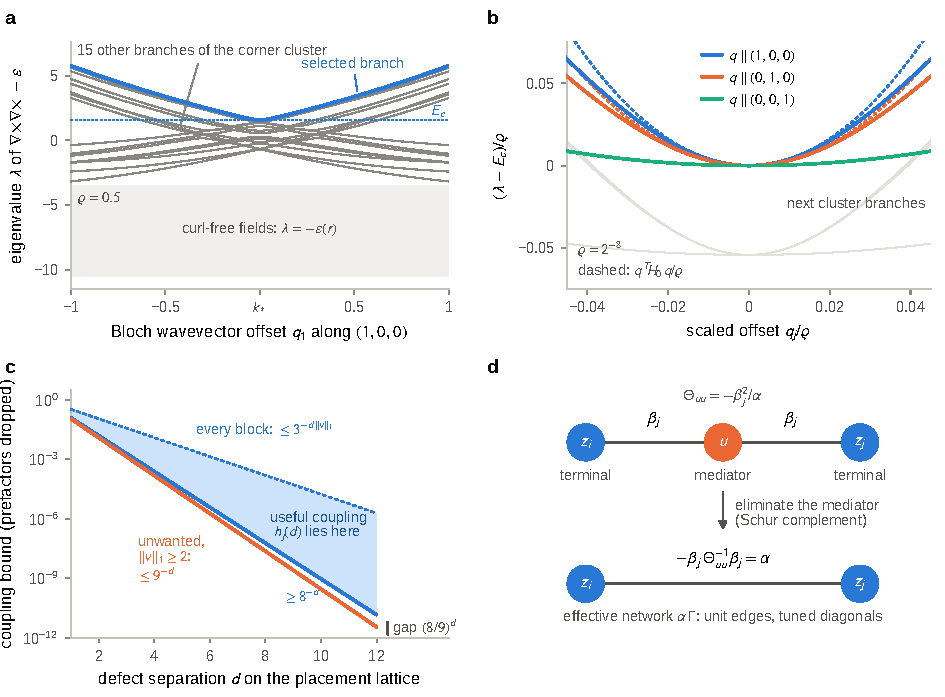
\includegraphics[width=\linewidth]{figures/fig2_mechanism.pdf}
\caption{\textbf{Broad defects in a weakly modulated dielectric interact like a network.}
\textbf{a}, Bloch spectrum of $\nabla\times\nabla\times-\varepsilon(x)$ for the periodic background
$\varepsilon=7+\delta\,[\cos\pi x_1+2\cos\pi x_2+4\cos\pi x_3]$ along the line $k=k_*+q_1(1,0,0)$
through $k_*=(\pi/2,\pi/2,\pi/2)$, computed with a vector plane-wave expansion (1029 plane-wave
components; eigenvalues converged to $10^{-7}$). The modulation is exaggerated to $\delta=0.5$ for
visibility; the construction uses $\delta=2^{-100}$. At $k_*$ eight plane waves of the unmodulated
medium are degenerate, forming a cluster of sixteen transverse branches that the modulation splits.
The selected branch (blue) is the highest of them and has an isolated local minimum $E_c$ at $k_*$.
Curl-free fields contribute the band $\lambda=-\varepsilon(x)$ (gray), and the other cluster branches
cross $E_c$ away from $k_*$: there is no complete gap, and the proof bounds leakage into these states
instead of assuming its absence.
\textbf{b}, The selected branch near $k_*$ along the three axes, computed at $\delta=2^{-8}$ and drawn
in scaled variables, in which the curves no longer change as $\delta\to0$. Dashed: the quadratic form
$q^{T}\!A_0\,q/\delta$ with the exact leading-order Hessian of the proof,
$A_0=\pi^2\,\mathrm{diag}(4.12,\,3.26,\,0.44)$; the next branches of the cluster (light gray) stay
$0.054\,\delta$ below the minimum.
\textbf{c}, Proven decay rates of the interaction between two defects $d$ placement-lattice steps
apart, with constant prefactors dropped: the useful nearest-neighbor coupling $h_j(d)$ is at least
$8^{-d}$ and, like every interaction block, at most $3^{-d}$, whereas every block between defects
that are not nearest neighbors is at most $9^{-d}$. The gap between the two rates is $(8/9)^{d}$:
because $9>8$, the summed unwanted couplings fall below the useful ones once $d=O(\log m)$.
\textbf{d}, A sign mediator $u$ between two terminals $z_i$, $z_j$ with couplings $\beta_j$ and tuned
self-term $T_{uu}=-\beta_j^2/\alpha$; eliminating it leaves the effective coupling $\alpha$, so the
defect amplitudes obey $\alpha\Gamma z=\alpha g$ for the compiled network matrix $\Gamma$, which has
unit edges and tuned diagonals.}
\label{fig:mechanism}
\end{figure}

% ---------------------------------------------------------------- Fig. 3
\begin{figure}[tbp]
\centering
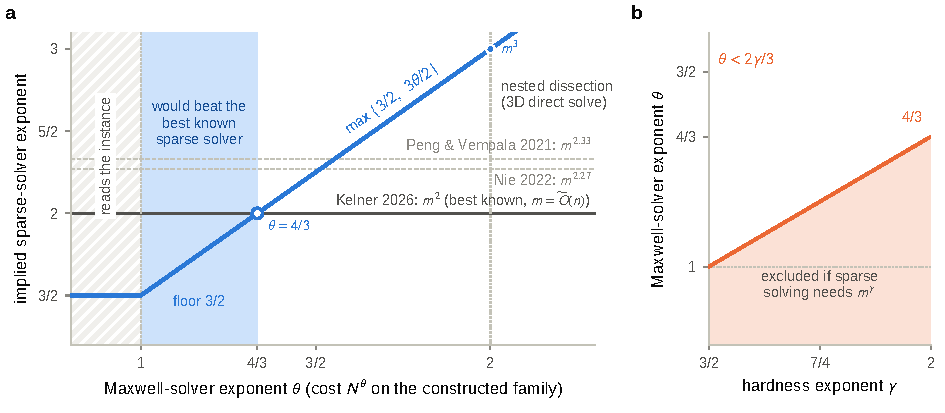
\includegraphics[width=\linewidth]{figures/fig3_consequence.pdf}
\caption{\textbf{What a fast Maxwell solver would mean for sparse linear algebra.}
\textbf{a}, If a solver handles every cavity of the constructed family in time $N^{\theta}$ up to
logarithmic factors, where $N$ counts grid cells and description length, then encoding, solving and
decoding solve every polynomially conditioned sparse system with $m$ nonzeros in time
$m^{\max\{3/2,\,3\theta/2\}}$ up to logarithmic factors (blue; the floor $3/2$ is the cost of encoding
and decoding). Horizontal lines are known bit-complexity upper bounds for the same problem class
($m=\widetilde O(n)$ nonzeros, polynomial condition number): the
$\widetilde O(mn\log(\kappa/\epsilon))$ algorithm of Kelner~\cite{kelner2026} gives $m^{2}$ and
supersedes the $m^{2.33}$ of Peng and Vempala~\cite{pengvempala2021,PengVempala2025} and the
$m^{2.27}$ of Nie~\cite{nie2022} (both stated with the matrix-multiplication exponent $\omega<2.3729$
used in those papers). Vertical
lines mark $\theta=1$, below which a solver can not read its input, and $\theta=2$, the cost of a
nested-dissection direct solve on a three-dimensional grid~\cite{George1973,LiptonRoseTarjan1979}. A
uniform solver with $1\le\theta<4/3$ (shaded) would improve the best known sparse-solver exponent.
The statement concerns worst-case solvers on this family of cavities; it says nothing about solvers
for other geometries or about typical instances.
\textbf{b}, Conversely, if solving sparse systems requires time $m^{\gamma}$ for some
$\gamma\in(3/2,2]$, the range compatible with the $m^{2}$ upper bounds (conjugate gradients in exact
arithmetic in the real-arithmetic model of the hypothesis; Kelner's algorithm in the bit model), no
uniform Maxwell solver for the family can have $\theta<2\gamma/3$ (shaded).}
\label{fig:consequence}
\end{figure}
 is not intended; copy each \caption into its figure environment.
% Cite keys refer to arxiv/references.bib.

% ---------------------------------------------------------------- Fig. 1
\begin{figure}[tbp]
\centering
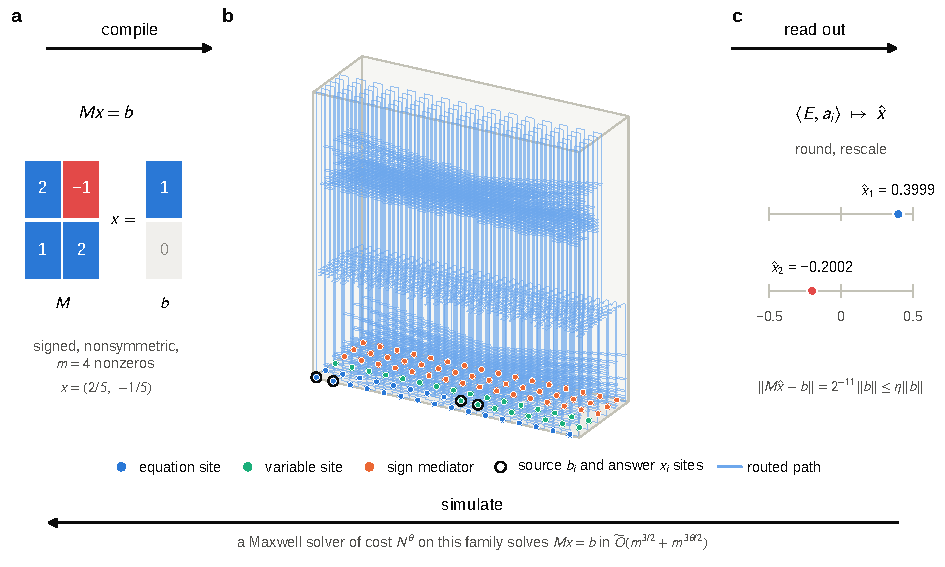
\includegraphics[width=\linewidth]{figures/fig1_concept.pdf}
\caption{\textbf{A sparse linear system and a dielectric cavity encode each other.}
\textbf{a}, The input is a sparse system $Mx=b$ with $m$ signed rational coefficients; shown is the
$2\times2$ example $M=\bigl(\begin{smallmatrix}2&-1\\1&2\end{smallmatrix}\bigr)$, $b=(1,0)$, whose
solution is $x=(2/5,\,-1/5)$. Blue and red cells are positive and negative entries.
\textbf{b}, The compiler expresses the equations through a local network of 96 sites (equation sites,
variable sites and sign mediators, each connected to at most three others) and routes its 96
connections as paths through a $505\times169\times3105$ integer grid. The drawing is the network the
compiler produced for the example in a, with the routing axis compressed sixfold for display; the paths
are long because the compiler equalizes their lengths. Each site becomes a broad, weak defect in the
periodic dielectric that fills the box, each path becomes a chain of such defects, and the walls are
perfect conductors. Ringed sites carry the source $b$ and the answer $x$.
\textbf{c}, A finite list of field moments $\langle E,a_i\rangle$ at the answer sites, rounded and
rescaled, returns $\hat x$. For the example, exact arithmetic on the compiled network gives
$\hat x=(819/2048,\,-205/1024)$ with relative residual $2^{-11}$, within the requested tolerance
$\eta=1/4$. Read from left to right (compile, read out), the cavity is an optical computer for $Mx=b$;
read from right to left (simulate), a Maxwell solver that handles this family of cavities in time
$N^{\theta}$, where $N$ counts grid cells, is a sparse linear solver of cost
$\widetilde O(m^{3/2}+m^{3\theta/2})$.}
\label{fig:concept}
\end{figure}

% ---------------------------------------------------------------- Fig. 2
\begin{figure}[tbp]
\centering
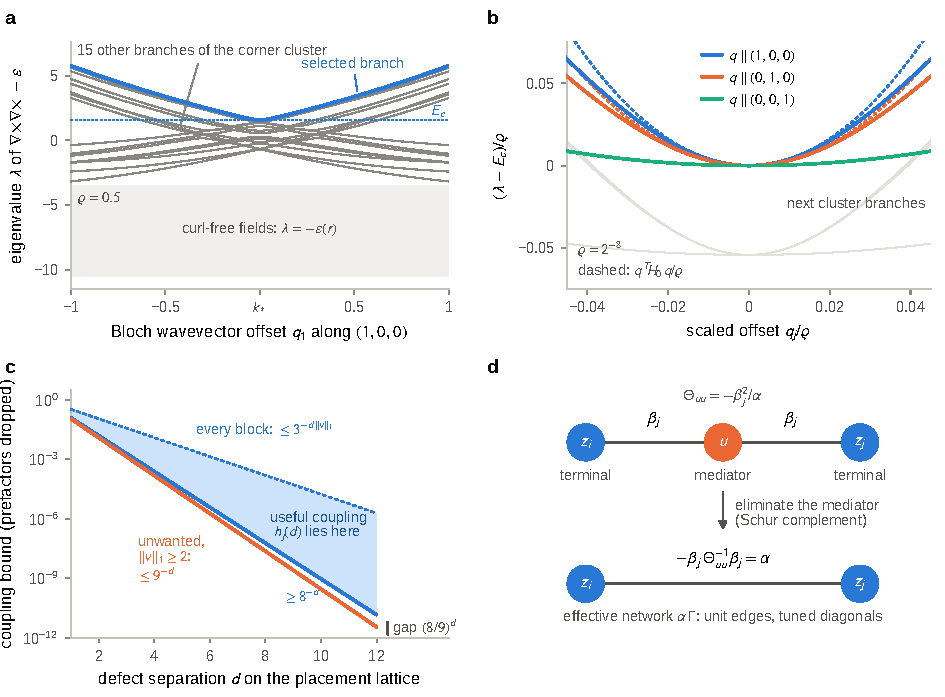
\includegraphics[width=\linewidth]{figures/fig2_mechanism.pdf}
\caption{\textbf{Broad defects in a weakly modulated dielectric interact like a network.}
\textbf{a}, Bloch spectrum of $\nabla\times\nabla\times-\varepsilon(x)$ for the periodic background
$\varepsilon=7+\delta\,[\cos\pi x_1+2\cos\pi x_2+4\cos\pi x_3]$ along the line $k=k_*+q_1(1,0,0)$
through $k_*=(\pi/2,\pi/2,\pi/2)$, computed with a vector plane-wave expansion (1029 plane-wave
components; eigenvalues converged to $10^{-7}$). The modulation is exaggerated to $\delta=0.5$ for
visibility; the construction uses $\delta=2^{-100}$. At $k_*$ eight plane waves of the unmodulated
medium are degenerate, forming a cluster of sixteen transverse branches that the modulation splits.
The selected branch (blue) is the highest of them and has an isolated local minimum $E_c$ at $k_*$.
Curl-free fields contribute the band $\lambda=-\varepsilon(x)$ (gray), and the other cluster branches
cross $E_c$ away from $k_*$: there is no complete gap, and the proof bounds leakage into these states
instead of assuming its absence.
\textbf{b}, The selected branch near $k_*$ along the three axes, computed at $\delta=2^{-8}$ and drawn
in scaled variables, in which the curves no longer change as $\delta\to0$. Dashed: the quadratic form
$q^{T}\!A_0\,q/\delta$ with the exact leading-order Hessian of the proof,
$A_0=\pi^2\,\mathrm{diag}(4.12,\,3.26,\,0.44)$; the next branches of the cluster (light gray) stay
$0.054\,\delta$ below the minimum.
\textbf{c}, Proven decay rates of the interaction between two defects $d$ placement-lattice steps
apart, with constant prefactors dropped: the useful nearest-neighbor coupling $h_j(d)$ is at least
$8^{-d}$ and, like every interaction block, at most $3^{-d}$, whereas every block between defects
that are not nearest neighbors is at most $9^{-d}$. The gap between the two rates is $(8/9)^{d}$:
because $9>8$, the summed unwanted couplings fall below the useful ones once $d=O(\log m)$.
\textbf{d}, A sign mediator $u$ between two terminals $z_i$, $z_j$ with couplings $\beta_j$ and tuned
self-term $T_{uu}=-\beta_j^2/\alpha$; eliminating it leaves the effective coupling $\alpha$, so the
defect amplitudes obey $\alpha\Gamma z=\alpha g$ for the compiled network matrix $\Gamma$, which has
unit edges and tuned diagonals.}
\label{fig:mechanism}
\end{figure}

% ---------------------------------------------------------------- Fig. 3
\begin{figure}[tbp]
\centering
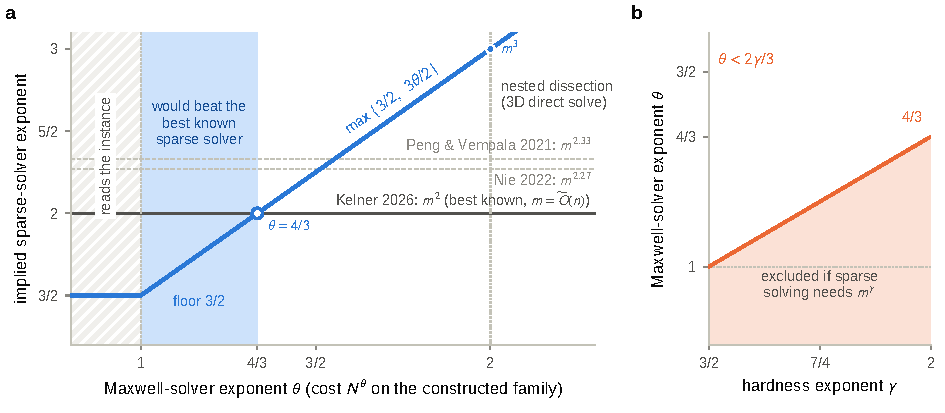
\includegraphics[width=\linewidth]{figures/fig3_consequence.pdf}
\caption{\textbf{What a fast Maxwell solver would mean for sparse linear algebra.}
\textbf{a}, If a solver handles every cavity of the constructed family in time $N^{\theta}$ up to
logarithmic factors, where $N$ counts grid cells and description length, then encoding, solving and
decoding solve every polynomially conditioned sparse system with $m$ nonzeros in time
$m^{\max\{3/2,\,3\theta/2\}}$ up to logarithmic factors (blue; the floor $3/2$ is the cost of encoding
and decoding). Horizontal lines are known bit-complexity upper bounds for the same problem class
($m=\widetilde O(n)$ nonzeros, polynomial condition number): the
$\widetilde O(mn\log(\kappa/\epsilon))$ algorithm of Kelner~\cite{kelner2026} gives $m^{2}$ and
supersedes the $m^{2.33}$ of Peng and Vempala~\cite{pengvempala2021,PengVempala2025} and the
$m^{2.27}$ of Nie~\cite{nie2022} (both stated with the matrix-multiplication exponent $\omega<2.3729$
used in those papers). Vertical
lines mark $\theta=1$, below which a solver can not read its input, and $\theta=2$, the cost of a
nested-dissection direct solve on a three-dimensional grid~\cite{George1973,LiptonRoseTarjan1979}. A
uniform solver with $1\le\theta<4/3$ (shaded) would improve the best known sparse-solver exponent.
The statement concerns worst-case solvers on this family of cavities; it says nothing about solvers
for other geometries or about typical instances.
\textbf{b}, Conversely, if solving sparse systems requires time $m^{\gamma}$ for some
$\gamma\in(3/2,2]$, the range compatible with the $m^{2}$ upper bounds (conjugate gradients in exact
arithmetic in the real-arithmetic model of the hypothesis; Kelner's algorithm in the bit model), no
uniform Maxwell solver for the family can have $\theta<2\gamma/3$ (shaded).}
\label{fig:consequence}
\end{figure}
